\section{Konečný stavový automat}
\noindent Existuje množstvo spôsobov ako modelovať správanie sytémov. Jedným z 
najstarších a najznámejších je modelovanie pomocou konečného stavového automatu.
Vďaka takejto abtrakcii môžeme o problémoch rozmýšľať ako o stavoch, ktoré nastali v určitom čase a charakterizujú to ako sa systém má správať. Táto technika však nieje limitovaná len na modelovanie softvérových systémov. Využíva sa aj v iných oblastiach ako napríklad vo fyzike a biológii \cite{WaybackMachine2014}. \par 
Konečný stavový automat je je výpočtový model, ktorý sa používa na simuláciu sekvenčnej logiky. Poznáme dva typy konečných stavových strojov: deterministický konečný automat (DKA)  a nedeterministický stavový automat (NKA) \cite{FiniteStateMachines}. 

\subsection{Deterministický konečný automat}
\noindent Deterministický konečný automat $\mathcal{M}$ je definovaný päticou ($\Sigma$ ,$\mathcal{Q}$ , $q_0$, $\mathcal{F}$, $\delta$) kde
\begin{itemize}
    \item $\Sigma$ je neprázdna a konečná vstupná abeceda $\mathcal{M}$
    \item $\mathcal{Q}$ je konečná množina stavov $\mathcal{M}$
    \item $q_0$ je počiatočný stav $\mathcal{M}$
    \item $\mathcal{F}$ $\subseteq$ $\mathcal{Q}$ je množina konečných stavov $\mathcal{M}$
    \item $\delta$ je prechodová funkcia  \begin{math}\delta : Q \times \Sigma \Rightarrow Q\end{math}
\end{itemize}

Automat musí definovať presne jednu prechodovú funkciu pre každý symbol v $\Sigma$ pre každý stav v $\mathcal{Q}$ \cite{FiniteStateMachines}. DKA môže byť reprenzentovaný pomocou diagramu ktorý vidíme na obrázku č.\ref{figure:dfa1}.

\begin{figure}[h]
    \centering
    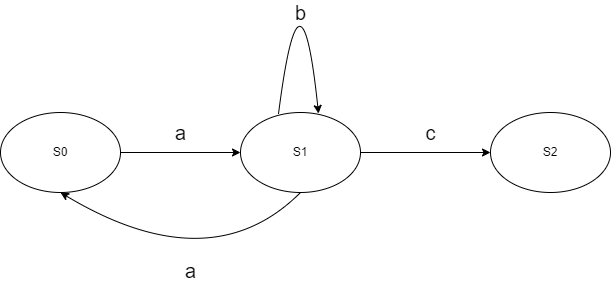
\includegraphics[width=0.70\textwidth]{img/dfa.png}
    \caption{Príklad deterministického konečného stavového automatu}
    \label{figure:dfa1}
\end{figure}

Rovnaký DKA môže byť popísaný aj nasledovne:
Nech $\mathcal{M}$ je pätica ($\Sigma$ ,$\mathcal{Q}$ , $q_0$, $\mathcal{F}$, $\delta$) kde, 

\begin{itemize}
    \item \begin{math} \Sigma = \{a, b ,c \}  \end{math}
    \item \begin{math} Q = \{S0, S1, S2 \}  \end{math}
    \item \begin{math} q_0 = \{S0 \}  \end{math}
    \item $\mathcal{F}$ \begin{math} = \{S2\}  \end{math}
\end{itemize}
a prechodová funkcia $\delta$ je daná tabuľkou číslo \ref{table:dfaPrechodovaFunckcia}:

\begin{table}[!htbp]    
    \begin{center}
    \begin{tabular}{c c|c}
    $\mathcal{Q}$ & $\Sigma$ & $\Rightarrow$ $\mathcal{Q}$  \\ \hline
    S0 & a & S1 \\ 
    S0 & b & S0 \\ 
    S0 & c & S0 \\ 
    S1 & a & S0 \\
    S1 & b & S1 \\  
    S1 & c & S2 \\  
    \end{tabular}
    \caption{Prechodová funkcia automatu $\mathcal{M}$}
    \label{table:dfaPrechodovaFunckcia}
    \end{center}
    \end{table}


\subsection{Nedeterministický konečný automat}
\noindent Podobne ako DKA aj NKA je reprenzentovaný ako  pätica ($\Sigma$ ,$\mathcal{Q}$ , $q_0$, $\mathcal{F}$, $\delta$) kde
\begin{itemize}
    \item $\Sigma$ je neprázdna a konečná vstupná abeceda $\mathcal{M}$
    \item $\mathcal{Q}$ je konečná množina stavov $\mathcal{M}$
    \item $q_0$ je počiatočný stav $\mathcal{M}$
    \item $\mathcal{F}$ $\subseteq$ $\mathcal{Q}$ je množina konečných stavov $\mathcal{M}$
    \item $\delta$ je prechodová funkcia  \begin{math}\delta : Q \times \Sigma \Rightarrow Q\end{math}
\end{itemize}

Narozdiel od DKA, NKA nevyžaduje definíciou prechodovej funkcie pre každý symbol 
patriaci $\Sigma$. Zároveň v NKA môže byť definovaná viac ako jedna prechodová funkcia $\delta$ pre symbol z $\Sigma$. Taktiež je možné použiť aj takzvané nulové prechody. Tie sa označujú ako $\epsilon$ a dovoľujú prechod z jedného stavu do druhého bez potreby prečítania akéhokoľvek symbolu patriaceho $\Sigma$ \cite{FiniteStateMachines}.